\subsection*{Question 1}
\begin{center}
	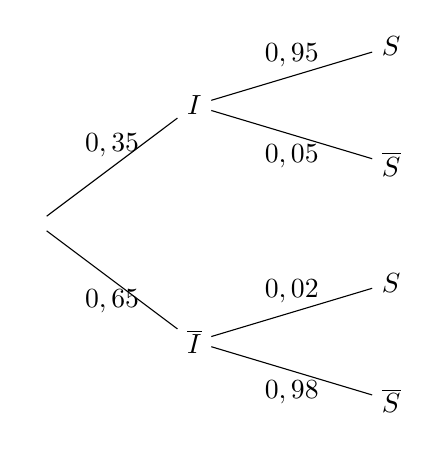
\begin{tikzpicture}
		[level 1/.style={level distance=2cm,
			sibling distance=3cm},
		level 2/.style={level distance=2.5cm,
			sibling distance=1.5cm}]
		\node {} [grow'=right]
		child {node {$I$}
			child {node {$S$}
				edge from parent node[above] {$0,95$}
			}
			child {node {$\overline S$}
				edge from parent node[below] {$0,05$}
			}
			edge from parent node[above] {$0,35$}
		}
		child {node {$\overline I$}
			child {node {$S$}
				edge from parent node[above] {$0,02$}
			}
			child {node {$\overline S$}
				edge from parent node[below] {$0,98$}
			}
			edge from parent node[below] {$0,65$}
		}
		;
	\end{tikzpicture}
\end{center}
\subsection*{Question 2}
On a 
\[
p\left(\overline{I} \cap S\right) = p\left(\overline{I}\right) \times p_{\overline{I}}(S) = 0{,}65 \times 0{,}02 = 0{,}013.
\]
\subsection*{Question 3}

D'après la loi des probabilités totales, on a :
\begin{align*}
	P(S) &= P(I \cap S) + P(\overline{I} \cap S).
\end{align*}
Or, $P(\overline{I} \cap S) = P(\overline{I}) \times P_{\overline{I}}(S) = 0,35 \times 0,95 = 0,3325$.\\
Donc :
\begin{align*}
	P(S) &= 0,3325 + 0,013 = 0,3455.
\end{align*}

\subsection*{Question 4}

On calcule $P_S(I)$ en utilisant la formule de Bayes :
\begin{align*}
	P_S(I) &= \frac{P(I \cap S)}{P(S)} \\
	&= \frac{0,3325}{0,3455} \approx 0,9623.
\end{align*}
Ainsi, $P_S(I) \approx 0,962$, arrondi au millième.

\subsection*{Question 5}

Le logiciel fait une erreur s'il ne bloque pas un courriel indésirable ou s'il bloque un courriel désirable. Cela correspond à la probabilité :
\begin{align*}
	P(\overline{I} \cap \overline{S}) + P(I \cap S) &= 0,35 \times 0,05 + 0,65 \times 0,02 \\
	&= 0,0175 + 0,013 = 0,0305.
\end{align*}
Donc, il y a environ 3,05\% de chance que le logiciel fasse une erreur, ce qui montre que le fournisseur ment.

